\documentclass[14pt]{beamer}
\usetheme{Pittsburgh}
\usepackage{xcolor}
\definecolor{USUBlue}{RGB}{26,57,89}
\usecolortheme[named=USUBlue]{structure}
\setbeamercolor{normal text}{fg=USUBlue}
\usepackage[utf8]{inputenc}
\usepackage{mathptmx}
\usepackage{tgbonum}
\usepackage{amssymb}
\usepackage{graphicx}
\usepackage{marvosym}
\usefonttheme{structuresmallcapsserif}
\usefonttheme{serif}
\setbeamercolor{author}{fg=USUBlue}
\setbeamerfont{author}{size=\small}
\setbeamerfont{frametitle}{size=\large}
\setbeamertemplate{enumerate items}[default]
\author{Elita Baldridge}
\title[17pt]{A data-intensive assessment of the species-abundance distribution.}
\setbeamertemplate{navigation symbols}{}
\date{}
%\setbeamercovered{transparent} 
%\logo{\includegraphics[scale=.03]{../Miscellaneous/Pictures/ecology_center_horizontal.jpg}\includegraphics[scale=0.07]{../Miscellaneous/Pictures/Weecology.png}} 
\institute{\includegraphics[scale=.07]{../Miscellaneous/Pictures/ecology_center_horizontal.jpg}\includegraphics[scale=0.1]{../Miscellaneous/Pictures/Weecology.png}} 
%\subject{} 
\begin{document}

\section{Title}
\begin{frame}[t]
\titlepage
\end{frame}

%\begin{frame}
%\tableofcontents
%\end{frame}

\section{Introduction}
\subsection{Commonness & rarity}
\begin{frame}[t]
\frametitle{Commonness \& rarity}
"Who can explain why one species ranges widely, and is very numerous, and why another allied species has a narrow range and is rare?  Yet these relations are of the highest important, for they determine the present welfare and, as I believe, the future success and modification of every inhabitant of this world."  


Darwin, 1859.

\note{
Few common species.
Many rare species.
One of the most fundamental and ubiquitous patterns in ecology.}
\end{frame}

\begin{frame}
Species abundance distribution
\begin{itemize}
\item Describes the distribution of commonness \& rarity of species.
\item Exhibits a hollow curve distribution.
\end{itemize}
\note{
Relative abundance distribution (RAD)
Species abundance distribution (SAD)}
\end{frame}

\subsection{What is macroecology?}
\begin{frame}[t]
\frametitle{Macroecology}
\normalsize One approach to studying ecological patterns and processes.\\
\begin{itemize}
\item Data intensive.
\item Large scales.
\begin{itemize}
\item Spatial
\item Temporal
\item Taxonomic
\end{itemize}
\item Search for generality.
\end{itemize}
\end{frame}

\begin{frame}
\frametitle{Macroecology}
\begin{Huge}
\begin{center}

Pattern 

\MVArrowDown{}  

Process  

\MVArrowDown{}
 
Prediction

\end{center}
\end{Huge}
\end{frame}

\subsection{Challenges of macroecology}
\begin{frame}[t]
\frametitle{Macroecology}
Challenges of macroecology\\
\begin{itemize}
\item Studies performed with a limited number of large datasets.
\item Lack of identification of pattern generating mechanisms.
\end{itemize}
\note{
Taxonomic and ecosystem limitations in datasets, e.g.North American terrestrial bias.}
\end{frame}

\subsection{Signal and Noise}
\begin{frame}[t]
\frametitle{Signal \& Noise}
\begin{center}
\includegraphics[scale=.4]{./sad-data/chapter3/SignalNoise.png}
\end{center}
\end{frame}


\subsection{Best practices}
\begin{frame}[t]
\frametitle{Macroecology}
Best practice recommendations\\
\begin{itemize}
\begin{small}
\item Test patterns with multiple taxonomic groups/ecosystems.  
\item Simultaneous testing of competing models and model predictions with a consistent statistical approach.
\end{small}
\end{itemize}
\end{frame}


\subsection{Introduction to Ecoinformatics}
\begin{frame}[t]
\frametitle{The Rules of Ecoinformatics}
\begin{Large}
Garbage in, garbage out.\\
\end{Large}
\begin{itemize}
\item All data are good, not all data are appropriate.
\item Fit the data to the question.
\end{itemize}
\end{frame}



\section{Data}
\subsection{Current Data}
\begin{frame}[t]
\frametitle{Data}
\vspace{-7pt}
\includegraphics[scale=.55]{./sad-data/chapter3/presentation_map.png}
\end{frame}

\begin{frame}[t]{}
\frametitle{Data}
\begin{large}
Major macroecological datasets\\
\end{large}
\begin{itemize}
\item Largely terrestrial
\item Largely North American
\item Many publicly available, some not.
\end{itemize}
~\\
~\\
~\\
~\\
\begin{large}
Lots of data in the literature.\\
\end{large}
\end{frame}


\subsection{Compiled Data}
\begin{frame}{}
\frametitle{Data}
\includegraphics[scale=.35]{../Miscellaneous/Pictures/Phd/CompiledData.png}
\end{frame}

\subsubsection{Data Collection}
\begin{frame}[shrink=30]
\frametitle{Data}
\begin{table}
\begin{tabular}{l|l} 
 Variable name & Variable definitions\\ 
\hline
 Class & Taxonomic class of species \\
 Family & Taxonomic family of species \\
 Genus & Taxonomic genus of species\\
 Species & Specific epithet of species  \\
 Relative\_abundance & Relative abundance of species \\
 Abundance & Abundance of species \\
 Collection\_Year & Start of collecting \\
 End\_Collection & End of collecting \\
 Site\_Name & Name/description of site \\
 Biogeographic\_region & Biogeographic region \\
 Site\_notes & Additional site information \\ 
\end{tabular}
\caption{List of variables collected.}
\end{table}
\end{frame}

\subsubsection{Data Summary}
\begin{frame}{}
\frametitle{Data}
\includegraphics[scale=.5]{./sad-data/dissertation/bioregions.png}
\end{frame}

\begin{frame}{}
\frametitle{Data}
\includegraphics[scale=.45]{./sad-data/dissertation/taxa_sites.png}
\end{frame}

\begin{frame}{}
\frametitle{Data}
\includegraphics[scale=.45]{./sad-data/dissertation/num_taxa.png}
\end{frame}

\subsection{Data Availability}
\begin{frame}[t]
\frametitle{Data}
~\\
~\\
The final community abundance database is publicly available and importable through the EcoData Retriever.\\ 
(http://www.ecodataretriever.org/)
\end{frame}

\section{The species abundance distribution}
\subsection{Pattern description}
\begin{frame}[t]{}
\frametitle{Commonness \& rarity}
~\\
\begin{large}
The species abundance distribution:
\end{large}
\begin{itemize}
\item Describes the distribution of commonness \& rarity of species.
\item One of the most fundamental and ubiquitous patterns in ecology.
\item Exhibits a hollow curve distribution.
\begin{itemize}
\item Many rare species.
\item Few common species.
~\\
\end{itemize}
\item Many forms of the species abundance distribution (SAD).
\end{itemize}
\end{frame}

\subsection{Forms of the distribution}
\begin{frame}
\frametitle{Forms of the SAD}
\begin{large}
Model classes:
\end{large}
\begin{itemize}
\item Purely statistical
\item Branching process
\item Population dynamics
\item Niche partitioning
\item Maximum entropy
\item Feasible set/combinatorics
\end{itemize}
\end{frame}
 

\section{Species abundance distribution comparisons}
\begin{frame}
\frametitle{SAD Comparisons}
\begin{large}
Most comparisons of the different models:
\end{large}
\begin{itemize}
\item Use only a small subset of available models (typically two).
\item Focus on a single ecosystem or taxonomic group
\item Fail to use the most appropriate statistical methods. 
\end{itemize}
\end{frame}

\subsection{Data & Analysis}
\subsubsection{Model selection}
\begin{frame}[shrink=10]
\frametitle{SAD Comparisons}
~\\
~\\
Selected five models from four classes for comparison.
\begin{table}
\begin{tabular}{l|l}
 Model class & Form of the distribution\\ 
\hline
 Purely statistical & Logseries, Poisson lognormal\\
 Branching process & Zipf \\
 Population dynamics & Negative binomial\\
 Niche partitioning & Geometric \\
\end{tabular}
~\\
~\\
~\\
~\\
\caption{After B.J. McGill et al. 2007. Species abundance distributions: moving beyond single prediction theories to integration within an ecological framework. Ecology letters 10: 995-1015.}
\end{table}
\end{frame}

\subsubsection{Analysis}
\begin{frame}
\frametitle{SAD Comparisons}
~\\
Analysis:
\begin{itemize}
\item Model fitting with maximum likelihood estimation. 
\item Likelihood based model selection to compare the fits of the different models.
\item Model comparison with corrected Aikaike Information Criterion (AICc) weights.
\end{itemize}
\end{frame}

\begin{frame}
\frametitle{SAD Comparisons}
~\\
Computational tools:
\begin{itemize}
\item Model fitting, log-likelihood, and AICc calculations performed with macroecotools Python package.\\
\begin{small}
(https://github.com/weecology/macroecotools)
\end{small}
\item All of the analysis code and the majority of the data is publicly available.
\begin{small}
(https://github.com/weecology/sad-comparison)
\end{small}
\end{itemize}
\end{frame}


\subsubsection{Data}
\begin{frame}[shrink=35]
\frametitle{SAD Comparisons}
\begin{center}
\begin{table}
\begin{tabular}{l|c|l|r}
 Dataset &Dataset code &Availability &Total sites\\
\hline
 Breeding Bird Survey &BBS &Public &2769\\
 Christmas Bird Count &CBC &Private &1999\\
 Gentry's Forest Transects &Gentry &Public &10355\\
 Forest Inventory Analysis &FIA	 &Public &220\\
 Mammal Community Database &MCDB &Public &103\\
 N. American Butterfly Count &NABA &Private &400\\
 Actinopterygii, this dissertation	 &Actinopterygii &Public &161\\
 Reptilia, this dissertation &Reptilia &Public &138\\
 Amphibia, this dissertation &Amphibia &Public &43\\
 Coleoptera, this dissertation &Coleoptera &Public &5\\
 Arachnida, this dissertation &Arachnida &Public &25\\
\end{tabular}
\caption{Datasets used for species-abundance distribution comparisons. Datasets marked as Private were obtained through data requests to the providers resulting in Memorandums of Understanding governing data use.}
\end{table}
\end{center}
\end{frame}

\begin{frame}{}
\frametitle{Data}
\includegraphics[scale=.4]{../Miscellaneous/Pictures/Phd/MapCreatures.png}
\end{frame}


\subsection{Results}
\begin{frame}{}
\frametitle{SAD Comparisons}
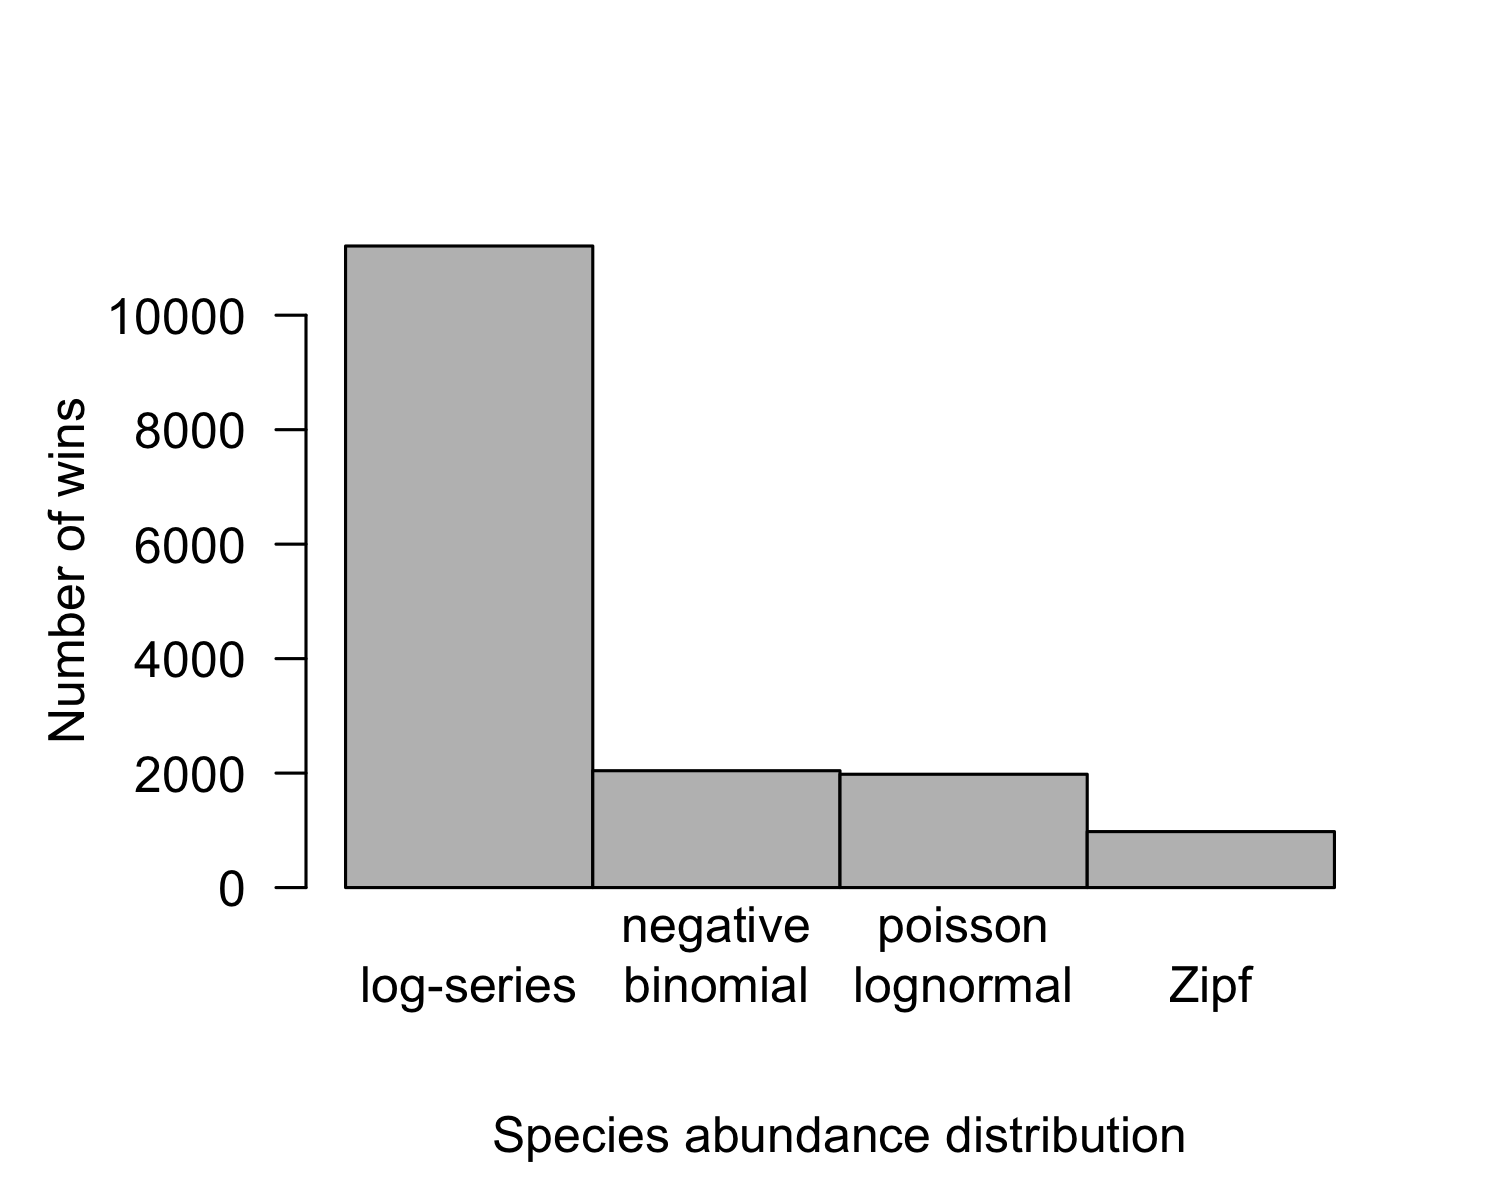
\includegraphics[scale=.5]{./sad-data/dissertation/total_wins.png}
\end{frame}

\begin{frame}{}
\frametitle{SAD Comparisons}
\includegraphics[scale=.40]{./sad-data/dissertation/wins_by_dataset.png}
\end{frame}

\begin{frame}{}
\frametitle{SAD Comparisons}
\includegraphics[scale=.5]{./sad-data/dissertation/AICc_weights.png}
\end{frame}

\begin{frame}{}
\frametitle{SAD Comparisons}
\includegraphics[scale=.5]{./sad-data/dissertation/likelihoods.png}
\end{frame}

\begin{frame}{}
\frametitle{SAD Comparisons}
\includegraphics[scale=.5]{./sad-data/dissertation/likelihoods_one_to_one.png}
\end{frame}

\subsection{Conclusions}
\begin{frame}
\frametitle{SAD Comparisons}
Existing models provide equivalently good absolute fits to empirical data.
\begin{itemize}
\item Models with fewer parameters perform better in AIC-based model selection.\\
\item Logseries provides a good naive model for fitting SADs.\\
\begin{itemize}
\item Produces equivalent likelihoods.
\item Has a single fitted parameter.
\item Easy to fit to empirical data.
\item Best overall model.
\end{itemize}
\end{itemize}
\end{frame}

\begin{frame}[t]
\frametitle{SAD Comparisons}
Identifying pattern generating mechanisms:
\begin{itemize}
\item Compare predictions of different models using multiple macroecological patterns simultaneously.\\
\item Examine scale dependence of pattern.
\end{itemize}
~\\
~\\
However, identification of mechanism may not be necessary for prediction.
\end{frame}

\section{Neutral analysis}
\begin{frame}[t]
\frametitle{Neutral Analysis}
~\\
The unified neutral theory of biodiversity:\\
~\\
\begin{itemize}
\item Multiple formulations.
\begin{itemize}
\item Species and individuals are ecologically and demographically equivalent.\\
\item Stochastic variation in birth, death, immigration, \& speciation results in species abundance differences.
\end{itemize}
\end{itemize}
\end{frame}

\begin{frame}
\frametitle{Neutral Analysis}
Early tests of neutral theory based on comparing the fit of empirical species abundance distributions to the neutral prediction.\\
~\\
Later tests suggested species abundance comparisons were insufficient for a rigorous test of neutrality.\\
~\\
\end{frame}

\begin{frame}
\frametitle{Neutral Analysis}
Connolly et al. 2014 identified non-neutral species abundance distributions in marine communities.\\
\begin{small}
\begin{itemize}
\item Compared model fits of a non-neutral distribution (Poisson lognormal) to a neutral distribution (negative binomial distribution).\\
\end{itemize}
\end{small}
~\\
May be a robust method for identifying communities that exhibit non-neutrality.\\
\begin{tiny}
S.R. Connolly et al. 2014. Commonness and rarity in the marine biosphere. PNAS 111: 8524-8529.
\end{tiny}
\end{frame}

\subsection{Data & Analysis}
\begin{frame}
\frametitle{Neutral Analysis}
Used the same data and model fitting approach.\\
Compared a non-neutral model (Poisson lognormal) to a neutral model (negative binomial).\\
\end{frame}

\begin{frame}{}
\frametitle{Neutral Analysis}
\includegraphics[scale=.43]{./sad-data/dissertation/EmpirModelHist.png}
\end{frame}

\subsection{Results}
\begin{frame}{}
\frametitle{Neutral Analysis}
\includegraphics[scale=.45]{./sad-data/dissertation/distabclasses_vs_lognormwgt.png}
\end{frame}

\begin{frame}{}
\frametitle{Neutral Analysis}
\includegraphics[scale=.40]{./sad-data/dissertation/avgvals_by_dataset.png}
\end{frame}

\subsection{Conclusions}
\begin{frame}
\frametitle{Neutral analysis}
Difficult to identify a clear winning model.
\begin{itemize}
\item Results consistent with our species abundance distribution model comparisons. 
\item Results different from Connolly et al. 2014.
\begin{itemize}
\item Non-neutral model outperforms the neutral model in marine systems.
\item Our results suggest marine systems more generally approximated by non-neutral dynamics; terrestrial systems more variable between neutral and non-neutral dynamics.
\end{itemize}
\end{itemize}
\end{frame}

\section{General Conclusions}
\begin{frame}{}
~\\ 
\frametitle{Conclusions}\
Challenging to infer process from species abundance distributions alone.
~\\ 
\begin{itemize}
\item Multiple mechanisms proposed for each SAD formulation.
\item Broad model categorization (i.e. neutral or non-neutral) may be more productive.
\item May not be one single suite of processes that dominates.
\end{itemize} 
\end{frame}

\begin{frame}[t]{}
\frametitle{Conclusions}\
~\\ 
Challenges in identifying mechanism among datasets.
~\\ 
\begin{itemize}
\item Biological vs. non-biological differences (spatial structuring, sampling intensity).
\item Diverse data removes uncertainty about non-biological pattern generating mechanisms.
\item Even with a great deal of data, identifying mechanism is still challenging.
\end{itemize} 
\end{frame}

\begin{frame}[t]{}
\frametitle{Conclusions}\
~\\ 
\begin{large}
Predictive macroecology
\end{large}
~\\ 
\begin{itemize}
\item Traditional approach is pattern to process to prediction.
\item May be possible to generate robust ecological predictions from general patterns.
\item Process and prediction may be two separate research goals.
\end{itemize} 
\end{frame}

\section{Acknowledgements}
\begin{frame}[t]{}
\frametitle{Acknowledgements}
~\\ %Adds vertical space for better aesthetics
\small{Funding sources:}
\begin{small}
\begin{itemize}
\item USU Department of Biology
\item Intellectual Ventures, private funding to Morgan Ernest
\item National Science Foundation CAREER Grant to Ethan White
\item Gordon \& Betty Moore Foundation's Data-Driven Discovery Initiative Grant to Ethan White.
\item USU Graduate School Dissertation Fellowship
\end{itemize}
\end{small}
\end{frame}

\begin{frame}{}
\frametitle{Acknowledgements}
Weecologists past, present, \& future\\
\includegraphics[scale=.3]{../Miscellaneous/Pictures/Phd/whiteboard.png}
\begin{tiny}
(especially Xiao Xiao \& Ken Locey (creator of the whiteboard))
\end{tiny}
\end{frame}

\begin{frame}[t]{}
\frametitle{Acknowledgements}
~\\ %Adds vertical space for better aesthetics
Dr. Thomas Price \& USU Student Health Center.\\
~\\
The Flint Hills of Kansas.\\
~\\
Tea, electric blankets, \& heating pads.\\
~\\
A very supportive husband \& family.\\
\end{frame}

\subsection{Accessibility}
\begin{frame}[t]{}
\frametitle{Accessibility}
\begin{center}
This dissertation brought to you by:
\end{center}
\begin{Large}
Disability accommodations\\
\end{Large}
~\\
\begin{itemize}
\item Remote access \& participation.\\
\item Computational tools \& tricks.
\begin{itemize}
\item Version control (GitHub).
\item Publicly available data.
\item Programming skills (data manipulation \& analysis).
\end{itemize}
\end{itemize}
\end{frame}

\section{Finis}
\begin{frame}[t]
\frametitle{Questions?}
\begin{center}
\includegraphics[scale=.28]{../Miscellaneous/Pictures/Maps/TheMaps.jpg}
\end{center}
\end{frame}

\end{document}